\documentclass[modern]{aastex61}

% All the packages
%\usepackage[letterpaper]{geometry}
\usepackage{microtype}
\usepackage{url}
\usepackage{amsmath}
\usepackage{mathtools}
\usepackage{esint}
\usepackage{amssymb}
\usepackage{natbib}
\usepackage{multirow}
\usepackage{graphicx}
\usepackage{scalerel}
\usepackage{calc}
\usepackage{etoolbox}
\usepackage{marginnote}
\usepackage{nicefrac}
\usepackage{tabstackengine}
\usepackage{diagbox}
\usepackage[makeroom]{cancel}
\usepackage{mathdots}
\usepackage{bbm}
\usepackage{booktabs}
\usepackage{xspace}
\stackMath

% Bibliography stuff
\bibliographystyle{aasjournal}

% Shorthand for this paper
\newcommand{\starry}{\textsf{starry}\xspace}

% References to text content
\newcommand{\documentname}{\textsl{article}}
\newcommand{\figureref}[1]{\ref{fig:#1}}
\newcommand{\Figure}[1]{Figure~\figureref{#1}}
\newcommand{\figurelabel}[1]{\label{fig:#1}}
\renewcommand{\eqref}[1]{\ref{eq:#1}}
\newcommand{\Eq}[1]{Equation~(\eqref{#1})}
\newcommand{\eq}[1]{\Eq{#1}}
\newcommand{\eqalt}[1]{Equation~\eqref{#1}}
\newcommand{\eqlabel}[1]{\label{eq:#1}}

% Add script hyperlinks as margin notes
\definecolor{proofcolor}{rgb}{0.1216,0.4667,0.7059}
\newcommand{\python}[1]{\marginnote{\href{https://github.com/rodluger/starry/tree/master/tex/figures/#1.py}{
\includegraphics[width=0.9cm]{figures/python.png}}}}
\newcommand{\mathematica}[1]{\marginnote{\href{https://github.com/rodluger/starry/tree/master/tex/notebooks/#1.nb}{
\includegraphics[width=0.6cm]{figures/mathematica.png}}}}
\newcommand{\todoproof}{\marginnote{\href{}{
\includegraphics[width=0.4cm]{figures/todo.png}}}}
\newcommand{\todo}[2]{\marginnote{\color{red}\textbf{#1:}\\\scriptsize\textbf{#2}}}

% Force margin notes to always be on the right side
% https://tex.stackexchange.com/a/69624

% Math stuff
\newcommand{\ii}{\ensuremath{\mathbf{i}}}
\newcommand{\T}{\ensuremath{\mathrm{T}}}
\newcommand{\dd}{\ensuremath{ \mathrm{d}}}
\newcommand{\unit}[1]{{\ensuremath{\mathrm{#1}}}}
\newcommand{\bvec}[1]{{\ensuremath{\mathbf{#1}}}}
\newcommand{\avec}[1]{{\ensuremath{\vec{\mathbf{#1}}}}}
\newcommand{\x}{\ensuremath{\mbox{$x$}}}
\newcommand{\y}{\ensuremath{\mbox{$y$}}}
\newcommand{\z}{\ensuremath{\mbox{$z$}}}
\newcommand{\xhat}{\ensuremath{\mathbf{\hat{x}}}}
\newcommand{\yhat}{\ensuremath{\mathbf{\hat{y}}}}
\newcommand{\zhat}{\ensuremath{\mathbf{\hat{z}}}}
\DeclareMathAlphabet\mathbfcal{OMS}{cmsy}{b}{n}
\DeclareMathOperator{\Tr}{Tr}
\DeclarePairedDelimiter\ceil{\lceil}{\rceil}
\DeclarePairedDelimiter\floor{\lfloor}{\rfloor}
\definecolor{dim}{rgb}{0.8,0.8,0.8}
\newcolumntype{L}[1]{>{\raggedright\let\newline\\\arraybackslash\hspace{0pt}}m{#1}}
\setcounter{MaxMatrixCols}{20}
\newcommand{\sinphi}{\ensuremath{\mbox{$u$}}}
\newcommand{\sinlambda}{\ensuremath{\mbox{$v$}}}
\newcommand{\bigdot}{\scaleto{\cdot}{6pt}}

% Bases
\newcommand{\pbasis}{\ensuremath{\bvec{\tilde{p}}}}
\newcommand{\gbasis}{\ensuremath{\bvec{\tilde{g}}}}
\newcommand{\ybasis}{\ensuremath{\bvec{\tilde{y}}}}
\newcommand{\pbasisn}{\ensuremath{\tilde{p}_n}}
\newcommand{\gbasisn}{\ensuremath{\tilde{g}_n}}
\newcommand{\ybasisn}{\ensuremath{\tilde{y}_n}}
\newcommand{\AOne}{\ensuremath{\bvec{A_1}}}
\newcommand{\ATwo}{\ensuremath{\bvec{A_2}}}

% Code examples
\usepackage{listings}
\definecolor{codegreen}{rgb}{0,0.6,0}
\definecolor{codegray}{rgb}{0.5,0.5,0.5}
\definecolor{codepurple}{rgb}{0.58,0,0.82}
\definecolor{backcolour}{rgb}{0.95,0.95,0.95}
\lstdefinestyle{mystyle}{
    backgroundcolor=\color{backcolour},
    commentstyle=\color{codegreen},
    keywordstyle=\color{magenta},
    numberstyle=\tiny\color{codegray},
    stringstyle=\color{codepurple},
    basicstyle=\small\ttfamily,
    breakatwhitespace=false,
    breaklines=true,
    captionpos=b,
    keepspaces=true,
    numbers=left,
    numbersep=5pt,
    showspaces=false,
    showstringspaces=false,
    showtabs=false,
    tabsize=2,
    aboveskip=1em,
    belowskip=1em
}
\lstset{style=mystyle}

% Inverse diagonal dots
\makeatletter
\def\Ddots{\mathinner{\mkern1mu\raise\p@
\vbox{\kern7\p@\hbox{.}}\mkern2mu
\raise4\p@\hbox{.}\mkern2mu\raise7\p@\hbox{.}\mkern1mu}}
\makeatother

% Typography obsessions
\setlength{\parindent}{3.0ex}
\renewcommand\quad{\hskip\fontdimen3\font}


\begin{document}\raggedbottom\sloppy\sloppypar\frenchspacing

\setlength{\abovedisplayskip}{1.5em}
\setlength{\belowdisplayskip}{1.5em}

\title{%
    \textbf{STARRY}: Analytic Occultation Light Curves
}

\author[0000-0002-0296-3826]{Rodrigo Luger}
\affil{Department~of~Astronomy, University~of~Washington, Seattle, WA}
\author{others}

\keywords{methods: analytical --- techniques: photometric}

\begin{abstract}
    We derive analytical, closed form solutions for the total flux
    emitted or reflected from a celestial body in the direction of
    an observer when the surface brightness map of the body is expressed
    as a sum of spherical harmonics.
    Our expressions apply to the computation of phase curves of stars and
    exoplanets, as well as to occultation light curves, including transits of
    planets across their host stars, occultations of planets by the star
    (secondary eclipses), and planet-planet and planet-moon occultations.
    We develop fast code in \textsf{C} that can be generally applied
    to any of these cases.
\end{abstract}

% ==============================================================================
% ------------------------------------------------------------------------------
% ------------------------------------------------------------------------------
%
\section{Introduction}
\label{sec:intro}
% ------------------------------------------------------------------------------
% ------------------------------------------------------------------------------
% ==============================================================================

Write a kick-ass intro here! \todo{RL}{write intro}

% ==============================================================================
% ------------------------------------------------------------------------------
% ------------------------------------------------------------------------------
\pagebreak
\section{Spherical harmonics}
\label{sec:spharm}
% ------------------------------------------------------------------------------
% ------------------------------------------------------------------------------
% ==============================================================================

The real spherical harmonic $Y_{lm}(\theta,\phi)$ of order $l$ and degree $m$
is defined in spherical coordinates as
%
\begin{align}
    \label{eq:ylmtp}
    Y_{lm}(\theta, \phi) =
    \begin{cases}
        \bar{P}_{lm}(\cos\theta)\cos(m\phi) & \qquad m \geq 0 \\
        \bar{P}_{l|m|}(\cos\theta)\sin(|m|\phi) & \qquad m < 0 \quad,
    \end{cases}
\end{align}
%
where $\bar{P}_{lm}$ is the normalized associated Legendre function. On the
surface of the unit sphere, we have
%
\begin{align}
    \label{eq:xyz}
    \x &= \sin\theta \cos\phi \nonumber \\
    \y &= \sin\theta \sin\phi \nonumber \\
    \z &= \cos\theta \quad.
\end{align}
%
Expanding Equation~(\ref{eq:ylmtp}) using the multiple angle formula, we obtain
%
\begin{align}
    \label{eq:ylm0}
    Y_{lm}(\x, \y , \z) =
    \left(\frac{1}{\sqrt{1 - \z^2}}\right)^m
    \begin{dcases}
        \bar{P}_{lm}(\z)
        \sum_{j\, \mathrm{even}}^{m}
        \left(-1\right)^\frac{j}{2}
        \binom{m}{j}
        \x^{m - j}
        \y^j
         & \qquad m \geq 0
         %
         \\[1em]
         %
        \bar{P}_{l|m|}(\z)
        \sum_{j\, \mathrm{odd}}^{m}
        \left(-1\right)^\frac{j-1}{2}
        \binom{m}{j}
        \x^{m - j}
        \y^j
        & \qquad m < 0 \quad ,
    \end{dcases}
\end{align}
%
where $\binom{\bigdot}{\bigdot}$ is the binomial
coefficient. The normalized associated Legendre function is defined as
%
\begin{align}
    \label{eq:plm}
    \bar{P}_{lm}(\z) &= A_{lm} \left(\sqrt{1-\z^2}\right)^m
                       \frac{\dd^m}{\dd \z^m}
                       \left[
                       \frac{1}{2^l l!}
                       \frac{\dd^l}{\dd \z^l}
                       \left(
                       \z^2 - 1
                       \right)^l
                       \right] \quad,
\end{align}
%
where
%
\begin{align}
    \label{eq:alm}
    A_{lm} = \sqrt{\frac{(2 - \delta_{m0})(2l + 1)(l - m)!}{4\pi(l + m)!}}
             \quad.
\end{align}
%
Expanding out the $\z$ derivatives, we obtain
%
\begin{align}
    \label{eq:plm_exp}
    \bar{P}_{lm}(\z) &= A_{lm} \left(\sqrt{1-\z^2}\right)^m\sum_{k=0}^{l-m}
                       \frac{2^l \left(\frac{l + m + k - 1}{2}\right)!}
                            {k!(l-m-k)!
                             \left(\frac{-l + m + k - 1}{2}\right)!}
                       \z^k
                       \quad,
\end{align}
%
which we combine with the previous results to write
%
\begin{align}
    \label{eq:ylmxyz}
    Y_{lm}(\x, \y , \z) &=
    \begin{dcases}
        \sum_{j\, \mathrm{even}}^m\sum_{k=0}^{l-m}
        \left(-1\right)^{\frac{j}{2}}
        A_{lm}
        B_{lm}^{jk}
        \x^{m - j}
        \y^j
        \z^k
        \qquad & m \ge 0 \\
        %
        \sum_{j\, \mathrm{odd}}^{|m|}\sum_{k=0}^{l-|m|}
        \left(-1\right)^{\frac{j-1}{2}}
        A_{l|m|}
        B_{l|m|}^{jk}
        \x^{|m| - j}
        \y^j
        \z^k
        \qquad & m < 0
    \end{dcases}
\end{align}
%
where
%
\begin{align}
    \label{eq:blmjk}
    B_{lm}^{jk} =
    \frac{2^l m! \left(\frac{l + m + k - 1}{2}\right)!}
         {j! k! (m - j)! (l - m - k)!
          \left(\frac{-l + m + k - 1}{2}\right)!} \quad.
\end{align}
%
\begin{figure}[t!]
    \begin{centering}
    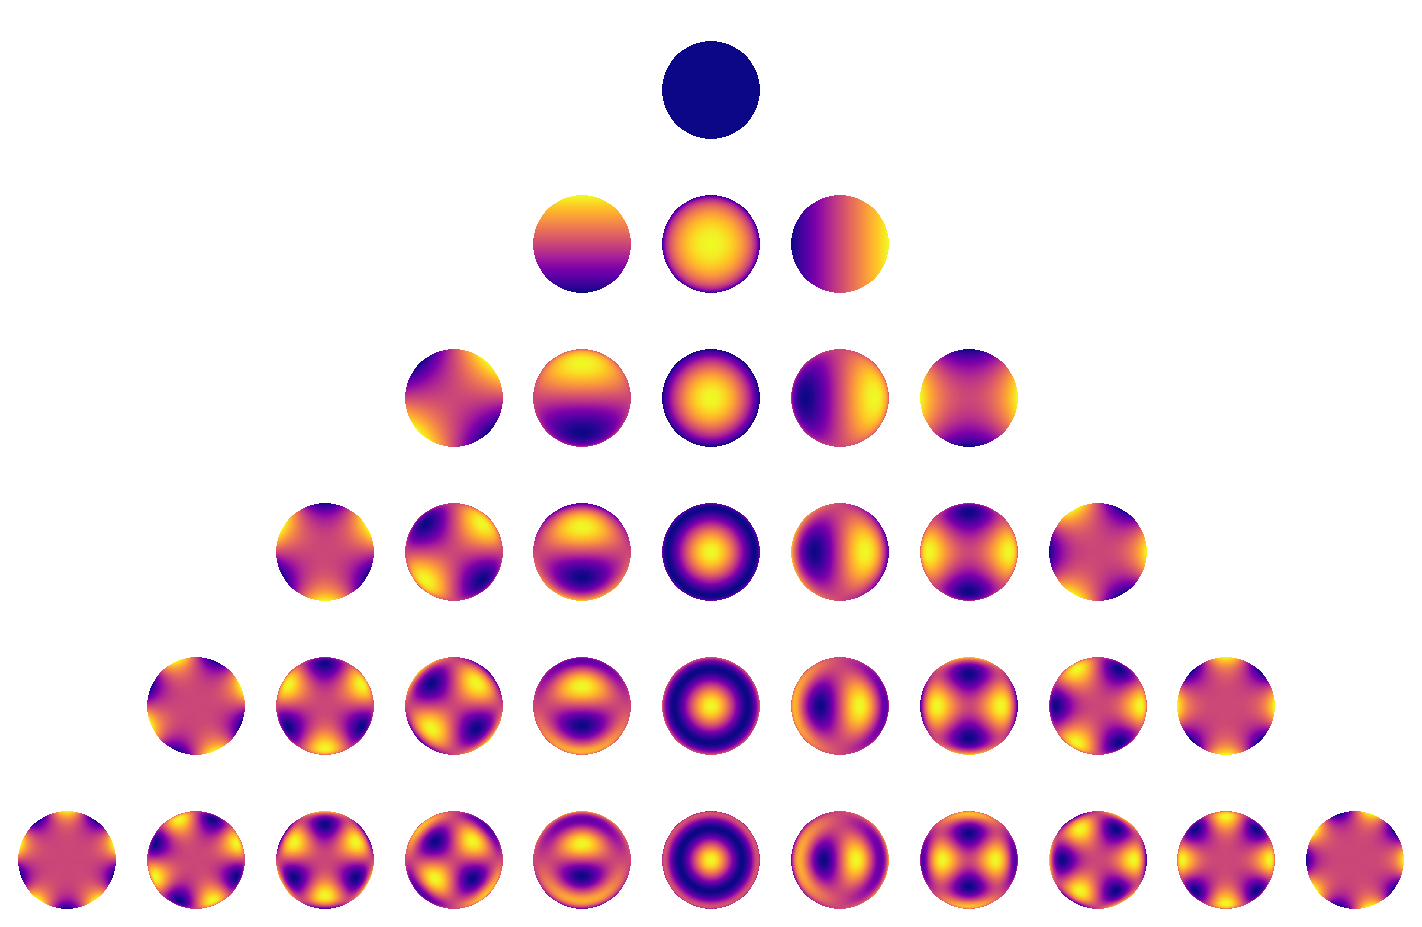
\includegraphics[width=\linewidth]{figures/ylms.pdf}
    \caption{\label{fig:ylms}
             \python{ylms}
             The real spherical harmonics up to order $l = 5$ computed from
             Equation~(\ref{eq:ylmxy}). In these plots, the $x$-axis points
             to the right, the $y$-axis points up, and the $z$-axis points
             out of the page. An animated version can be viewed
             \href{https://raw.githubusercontent.com/rodluger/%
                   cartograpy/gif/ylms.gif}{here}.}
    \end{centering}
\end{figure}
%
Since we are confined to the surface of the unit sphere, we have
$\z = \sqrt{1 - \x^2 - \y^2}$ and we may expand $\z^k$ using
the binomial theorem:
%
\begin{align}
    \z^{k} &= (1 - \x^2 - \y^2)^\frac{k}{2} \nonumber \\[0.5em]
          &=
          \begin{dcases}
              \sum_{p\,\mathrm{even}}^{k}
              \sum_{q\,\mathrm{even}}^p
              (-1)^\frac{p}{2}
              C_{pq}^{k}
              \x^{p-q} \y^{q}
              \qquad & k\,\mathrm{even} \\
              %
              \sum_{p\,\mathrm{even}}^{k - 1}
              \sum_{q\,\mathrm{even}}^p
              (-1)^\frac{p}{2}
              C_{pq}^{k-1}
              \x^{p-q} \y^{q} \sqrt{1 - \x^2 - \y^2}
              \qquad & k\,\mathrm{odd} \quad,
          \end{dcases}
          \label{eq:zk}
\end{align}
%
where
%
\begin{align}
    \label{eq:ckpq}
    C_{pq}^{k} =
    \frac{\left(\frac{k}{2}\right)!}{\left(\frac{q}{2}\right)!
    \left(\frac{k-p}{2}\right)! \left(\frac{p-q}{2}\right)!} \quad.
\end{align}
%
This gives us an expression for the spherical harmonic $Y_{lm}$
as a function of $\x$ and $\y$ only:
%
\begin{align}
    \label{eq:ylmxy}
    Y_{lm}(\x, \y) &=
    \begin{dcases}
        \!\begin{aligned}%[b]
            &
                \sum_{j\, \mathrm{even}}^m
                \sum_{k\, \mathrm{even}}^{l-m}
                \sum_{p\,\mathrm{even}}^{k}
                \sum_{q\,\mathrm{even}}^p
                \left(-1\right)^{\frac{j+p}{2}}
                A_{lm}
                B_{lm}^{jk}
                C_{pq}^{k}
                \x^{m - j + p - q}
                \y^{j + q}
            \, + \\
            &
                \sum_{j\, \mathrm{even}}^m
                \sum_{k\, \mathrm{odd}}^{l-m}
                \sum_{p\,\mathrm{even}}^{k - 1}
                \sum_{q\,\mathrm{even}}^p
                \left(-1\right)^{\frac{j+p}{2}}
                A_{lm}
                B_{lm}^{jk}
                C_{pq}^{k - 1}
                \x^{m - j + p - q}
                \y^{j + q}
                \z
       \end{aligned}
       &
       \quad m \ge 0 \\
       %
       %
       \\
       %
       %
       \!\begin{aligned}%[b]
           &
               \sum_{j\, \mathrm{odd}}^{|m|}
               \sum_{k\, \mathrm{even}}^{l-|m|}
               \sum_{p\,\mathrm{even}}^{k}
               \sum_{q\,\mathrm{even}}^p
               \left(-1\right)^{\frac{j+p-1}{2}}
               A_{l|m|}
               B_{l|m|}^{jk}
               C_{pq}^{k}
               \x^{|m| - j + p - q}
               \y^{j + q}
           \, + \\
           &
               \sum_{j\, \mathrm{odd}}^{|m|}
               \sum_{k\, \mathrm{odd}}^{l-|m|}
               \sum_{p\,\mathrm{even}}^{k - 1}
               \sum_{q\,\mathrm{even}}^p
               \left(-1\right)^{\frac{j+p-1}{2}}
               A_{l|m|}
               B_{l|m|}^{jk}
               C_{pq}^{k - 1}
               \x^{|m| - j + p - q}
               \y^{j + q}
               \z
      \end{aligned}
      &
      \quad m < 0
   \end{dcases}
    %
\end{align}
%
where $\z = \z(\x, \y) = \sqrt{1 - \x^2 - \y^2}$.

% ==============================================================================
% ------------------------------------------------------------------------------
% ------------------------------------------------------------------------------
\pagebreak
\section{Surface map vectors}
\label{sec:vectors}
% ------------------------------------------------------------------------------
% ------------------------------------------------------------------------------
% ==============================================================================

We represent a surface map as a vector $\bvec{y}$ of spherical harmonic
coefficients such that the specific intensity at the point
$(\x, \y)$ may be written
%
\begin{align}
    \label{eq:I}
    I(\x, \y) = \ybasis^\mathsf{T} (\x, \y) \, \bvec{y}
    \quad,
\end{align}
%
where $\ybasis$ is the basis of spherical harmonics,
arranged in increasing degree and order:
%
\begin{align}
    \label{eq:by}
    \ybasis =
    \begin{pmatrix}
        Y_{0, 0} &
        Y_{1, -1} & Y_{1, 0} & Y_{1, 1} &
        Y_{2, -2} & Y_{2, -1} & Y_{2, 0} & Y_{2, 1} & Y_{2, 2} &
        \cdot\cdot\cdot
    \end{pmatrix}^\mathsf{T}
    \quad,
\end{align}
%
where $Y_{l, m} = Y_{l, m}(\x, \y)$ are given by \eq{ylmxy}.
For reference, in this basis the coefficient of the spherical harmonic
$Y_{l, m}$ is located at the index
%
\begin{align}
    \label{eq:n}
    n = l^2 + l + m
\end{align}
%
of the vector $\bvec{y}$. Conversely, the coefficient at index $n$
of $\bvec{y}$ corresponds
to the spherical harmonic of order and degree given by
%
\begin{align}
    \label{eq:lm}
    l &= \floor*{\sqrt{n}} \nonumber \\
    m &= n - \floor*{\sqrt{n}}^2 - \floor*{\sqrt{n}}
    \quad.
\end{align}
%

% ==============================================================================
% ------------------------------------------------------------------------------
% ------------------------------------------------------------------------------
\pagebreak
\section{Rotation}
\label{sec:rotation}
% ------------------------------------------------------------------------------
% ------------------------------------------------------------------------------
% ==============================================================================

% ------------------------------------------------------------------------------
\subsection{Euler angles}
\label{sec:euler}
% ------------------------------------------------------------------------------

Defining a map as a vector of spherical harmonic coefficients makes it
straightforward to compute the projection of the map under arbitrary rotations
of the body via a rotation matrix $\bvec{R}$:
%
\begin{align}
    \label{eq:rotation}
    \bvec{y'} = \bvec{R} \, \bvec{y}
\end{align}
%
where $\bvec{y'}$ are the spherical harmonic coefficients of the rotated map.
\citet{AlvarezCollado1989} derived expressions for the rotation matrices for
the real spherical harmonics of a given order $l$ from the corresponding
complex rotation matrices \citep{Steinborn1973}:
%
\begin{align}
    \label{eq:rl}
    \bvec{R}^l = \bvec{U}^{-1} \bvec{D}^l \bvec{U}
\end{align}
%
where
%
\begin{align}
    \label{eq:dl}
    \bvec{D}^l_{m,m'} &= \mathrm{e}^{-\ii (\alpha m' + \gamma m)}
                       (-1)^{m' + m}
                       \sqrt{
                            (l - m)! (l + m)! (l - m')! (l + m')!
                       }
                       \nonumber \\
                       & \phantom{=}
                       \times
                       \sum_k (-1)^k
                              \frac{
                                \cos\left(\frac{\beta}{2}\right)^{2l + m - m' - 2k}
                                \sin\left(\frac{\beta}{2}\right)^{-m + m' + 2k}
                              }{
                                k! (l + m - k)! (l - m' - k)! (m' - m + k)!
                              }
\end{align}
%
is the rotation matrix for the complex spherical harmonics of order $l$ and
%
\begin{equation}
    \label{eq:U}
    \setstackgap{L}{1.25\baselineskip}
    \fixTABwidth{T}
    \bvec{U} =
    \frac{1}{\sqrt{2}}
        \parenMatrixstack{
            \quad\quad\, \ddots \, \quad\quad\quad\quad
                   &     &     &     &          &     &     &     & \Ddots \\
                   & \ii &     &     &          &     &     &  1  &        \\
                   &     & \ii &     &          &     &  1  &     &        \\
                   &     &     & \ii &          &  1  &     &     &        \\
                   &     &     &     & \sqrt{2} &     &     &     &        \\
                   &     &     & \ii &          &  1  &     &     &        \\
                   &     & \ii &     &          &     &  1  &     &        \\
                   & \ii &     &     &          &     &     &  1  &        \\
            \Ddots &     &     &     &          &     &     &     & \ddots
        }\quad.
\end{equation}
%
describes the transformation from complex to real spherical harmonics. In
\eq{dl} above, $\alpha$, $\beta$, and $\gamma$ are the (proper) Euler angles
for rotation in the $z-y-z$ convention.
%
To obtain a rotation matrix for an arbitrary vector $\bvec{y}$ with spherical
harmonics of different orders up to $l = l_\mathrm{max}$, we define the
block-diagonal matrix $\bvec{R}$:
%
\begin{equation}
    \label{eq:rblockdiag}
    \setstackgap{L}{1.25\baselineskip}
    \fixTABwidth{T}
    \bvec{R} =
        \parenMatrixstack{
            \quad\quad \, \bvec{R}^0 \, \quad\quad
                       &            &            &            &  \\
                       & \bvec{R}^1 &            &            &  \\
                       &            & \bvec{R}^2 &            &  \\
                       &            &            & \bvec{R}^3 &  \\
                       &            &            &            & \ddots
        }\quad.
\end{equation}
%
Rotation of $\bvec{y}$ by the Euler angles $\alpha$, $\beta$, and $\gamma$
is performed via \eq{rotation} with $\bvec{R}$ given by \eq{rblockdiag}.

% ------------------------------------------------------------------------------
\subsection{Axis-angle}
\label{sec:axisangle}
% ------------------------------------------------------------------------------

It is often more convenient to define a rotation by an axis $\bvec{u}$
and an angle $\theta$ of rotation about that axis. Given a unit vector
$\bvec{u}$ and an angle $\theta$, we can find the corresponding Euler
angles by comparing the 3-dimensional Cartesian rotation matrices for
both systems,
%
\begin{equation}
    \label{eq:rotP}
    \setstackgap{L}{1.25\baselineskip}
    \fixTABwidth{T}
    \mathbf{P} =
        \parenMatrixstack{
        c_\theta + u_x^2 \left(1 - c_\theta\right)
        &
        u_x u_y \left(1 - c_\theta\right) - u_z s_\theta
        &
        u_x u_z \left(1 - c_\theta\right) + u_y s_\theta
        \\
        u_y u_x \left(1 - c_\theta\right) + u_z s_\theta
        &
        % Add a little padding
        \makebox[1.5em]{}
        c_\theta + u_y^2\left(1 - c_\theta\right)
        \makebox[1.5em]{}
        &
        u_y u_z \left(1 - c_\theta\right) - u_x s_\theta
        \\
        u_z u_x \left(1 - c_\theta\right) - u_y s_\theta
        &
        u_z u_y \left(1 - c_\theta\right) + u_x s_\theta
        &
        c_\theta + u_z^2\left(1 - c_\theta\right)
        }
\end{equation}
%
for axis-angle rotations and
%
\begin{equation}
    \label{eq:rotQ}
    \setstackgap{L}{1.25\baselineskip}
    \fixTABwidth{T}
    \mathbf{Q} =
        \parenMatrixstack{
        c_\alpha c_\beta c_\gamma - s_\alpha s_\gamma
        &
        -c_\gamma s_\alpha - c_\alpha c_\beta s_\gamma
        &
        c_\alpha s_\beta
        \\
        c_\alpha s_\gamma + c_\beta c_\gamma s_\alpha
        &
        c_\alpha c_\gamma - c_\beta s_\alpha s_\gamma
        &
        s_\alpha s_\beta
        \\
        -c_\gamma s_\beta
        &
        s_\beta s_\gamma
        &
        \makebox[4.2em]{}
        c_\beta
        \makebox[4.2em]{}
        }\quad,
\end{equation}
%
for Euler rotations,
where $c_{\bigdot} \equiv \cos(\cdot)$
and $s_{\bigdot} \equiv \sin(\cdot)$.
Comparison of the two matrices gives us expressions for the Euler
angles in terms of $\bvec{u}$ and $\theta$:
%
\begin{align}
    \label{eq:eulerangles}
    \begin{matrix}
        \cos\alpha = \frac{P_{0,2}}{\sqrt{P_{0,2}^2 + P_{1,2}^2}}
        & & & &
        \cos\beta = P_{3,3}
        & & & &
        \cos\gamma = -\frac{P_{2,0}}{\sqrt{P_{2,0}^2 + P_{2,1}^2}}
        \\
        \sin\alpha = \frac{P_{1,2}}{\sqrt{P_{0,2}^2 + P_{1,2}^2}}
        & & & &
        \sin\beta = \sqrt{1 - P_{3,3}^2}
        & & & &
        \sin\gamma = \frac{P_{2,1}}{\sqrt{P_{2,0}^2 + P_{2,1}^2}}
    \end{matrix}
    \quad.
\end{align}
%
Thus, given a spherical harmonic vector $\bvec{y}$, we can calculate
how it transforms under rotation by an angle $\theta$ about an axis $\bvec{u}$
by first computing the Euler angles (Equation~\ref{eq:eulerangles}) and using
those to construct the spherical harmonic rotation matrix
(Equation~\ref{eq:rblockdiag}).

% ==============================================================================
% ------------------------------------------------------------------------------
% ------------------------------------------------------------------------------
\pagebreak
\section{Change of basis}
\label{sec:basis}
% ------------------------------------------------------------------------------
% ------------------------------------------------------------------------------
% ==============================================================================

% ------------------------------------------------------------------------------
\subsection{Polynomial basis}
\label{sec:polybasis}
% ------------------------------------------------------------------------------

In order to compute the occultation light curve for a body with a given surface
map $\bvec{y}$, it is convenient to first find its polynomial representation
$\bvec{p}$, which we express as a vector of coefficients in the
polynomial basis $\pbasis$:
%
\begin{align}
    \label{eq:bp}
    \pbasisn &=
    \begin{dcases}
        \x^\frac{\mu}{2} \y^\frac{\nu}{2} & \qquad \nu \, \mathrm{even}
        \\
        \x^\frac{\mu-1}{2} \y^\frac{\nu-1}{2} \z & \qquad \nu \, \mathrm{odd}
    \end{dcases}
    \nonumber\\[0.5em]
    \pbasis &=
    \begin{pmatrix}
        1 &
        \x & \z & \y &
        \x^2 & \x\z & \x\y & \y\z & \y^2 &
        \cdot\cdot\cdot
    \end{pmatrix}^\mathsf{T}
    \quad,
\end{align}
%
where
%
\begin{align}
    \label{eq:munu}
    \mu &= l - m \nonumber \\
    \nu &= l + m
    \quad
\end{align}
%
with $l$ and $m$ given by \eq{lm}.
%
%
To find $\bvec{p}$ given $\bvec{y}$, we
introduce the change of basis matrix $\AOne$,
which transforms
a vector in the spherical harmonic basis $\ybasis$ to the
polynomial basis $\pbasis$:
%
\begin{align}
    \bvec{p} = \AOne \, \bvec{y}
\end{align}
%
The columns of $\AOne$ are simply the polynomial vectors
corresponding to each of the spherical harmonics in \eq{by}. From
Equations (\ref{eq:ylmxy}) and (\ref{eq:bp}), we can calculate
the first few spherical harmonics and their corresponding polynomial vectors:
%
\begin{equation}
\def\arraystretch{1.3}
\begin{array}{@{}lcccccccl@{}}
    \phantom{..}
    Y_{0,0} = \frac{1}{2\sqrt{\pi}}
    & & & & & & & &
    \bvec{p} = \frac{1}{2\sqrt{\pi}}
                  \begin{pmatrix}
                        1 & 0 & 0 & 0 & \cdot\cdot\cdot
                  \end{pmatrix}^\mathsf{T}
    %
    \\
    %
    Y_{1,-1} = \frac{\sqrt{3}}{2\sqrt{\pi}}\y
    & & & & & & & &
    \bvec{p} = \frac{1}{2\sqrt{\pi}}
                  \begin{pmatrix}
                        0 & 0 & 0 & \sqrt{3} & \cdot\cdot\cdot
                  \end{pmatrix}^\mathsf{T}
    %
    \\
    %
    \phantom{..}
    Y_{1,0} = \frac{\sqrt{3}}{2\sqrt{\pi}}\z
    & & & & & & & &
    \bvec{p} = \frac{1}{2\sqrt{\pi}}
                \begin{pmatrix}
                      0 & 0 & \sqrt{3} & 0 & \cdot\cdot\cdot
                \end{pmatrix}^\mathsf{T}
    %
    \\
    %
    \phantom{..}
    Y_{1,1} = \frac{\sqrt{3}}{2\sqrt{\pi}}\x
    & & & & & & & &
    \bvec{p} = \frac{1}{2\sqrt{\pi}}
                  \begin{pmatrix}
                        0 & \sqrt{3} & 0 & 0 & \cdot\cdot\cdot
                  \end{pmatrix}^\mathsf{T}
    %
    \\
    %
    Y_{2,-2} = \cdot\cdot\cdot
    & & & & & & & &
    \bvec{p} = \cdot\cdot\cdot
\end{array}
\end{equation}
%
From these we can construct $\AOne$. As an example, for spherical
harmonics up to order $l_\mathrm{max} = 3$, this is
%
\begin{equation}
    \setstackgap{L}{1.25\baselineskip}
    \fixTABwidth{T}
    \AOne =
    \frac{1}{2 \sqrt{\pi }}
        \parenMatrixstack{
            1 & 0 & 0 & 0 & 0 & 0 & \sqrt{5} & 0 & 0 \\
            0 & 0 & 0 & \sqrt{3} & 0 & 0 & 0 & 0 & 0 \\
            0 & 0 & \sqrt{3} & 0 & 0 & 0 & 0 & 0 & 0 \\
            0 & \sqrt{3} & 0 & 0 & 0 & 0 & 0 & 0 & 0 \\
            0 & 0 & 0 & 0 & 0 & 0 & -\frac{3 \sqrt{5}}{2} & 0 & \frac{\sqrt{15}}{2} \\
            0 & 0 & 0 & 0 & 0 & 0 & 0 & \sqrt{15} & 0 \\
            0 & 0 & 0 & 0 & \sqrt{15} & 0 & 0 & 0 & 0 \\
            0 & 0 & 0 & 0 & 0 & \sqrt{15} & 0 & 0 & 0 \\
            0 & 0 & 0 & 0 & 0 & 0 & -\frac{3 \sqrt{5}}{2} & 0 & -\frac{\sqrt{15}}{2}
        }\quad.
    \mathematica{A1}
\end{equation}
%
As before, the specific intensity at the point $(\x, \y)$
may be computed as
%
\begin{align}
    I(\x, \y) &= \pbasis^\mathsf{T} \bvec{p} \nonumber \\
              &= \pbasis^\mathsf{T} \AOne \, \bvec{y}
    \quad.
\end{align}

% ------------------------------------------------------------------------------
\subsection{Green's basis}
\label{sec:greensbasis}
% ------------------------------------------------------------------------------

As we will see in the next section, integrating the surface map over the disk of
the body is easier if we apply one final transformation to our input vector,
rotating it into what we will refer to as the \emph{Green's basis}, $\gbasis$:
%
\begin{align}
    \label{eq:bg}
    \gbasisn &=
    \begin{dcases}
        %
        \frac{\mu+2}{2}\x^\frac{\mu}{2} \y^\frac{\nu}{2}
            & \qquad \nu \, \mathrm{even}
        \\[1em]
        %
        \z
            & \qquad \nu = \mu = 1
        \\[1em]
        %
        3\x^{l-2}\y\z
            & \qquad \nu \, \mathrm{odd}, \,
                     \mu = 1, \,
                     l \, \mathrm{even}
        \\[1em]
        %
        \z
        \bigg(
         -\x^{l-3} + \x^{l-1} + 4\x^{l-3}\y^2
        \bigg)
         & \qquad \nu \, \mathrm{odd}, \,
                  \mu = 1, \,
                  l \, \mathrm{odd}
        \\[1em]
        %
        \z
        \bigg(
            \frac{\mu-3}{2} \x^\frac{\mu-5}{2} \y^\frac{\nu-1}{2}
            -
            \frac{\mu-3}{2} \x^\frac{\mu-5}{2} \y^\frac{\nu+3}{2}
            -
            \frac{\mu+3}{2} \x^\frac{\mu-1}{2} \y^\frac{\nu-1}{2}
        \bigg)
            & \qquad \mathrm{otherwise}
    \end{dcases}
    \nonumber\\[1.5em]
    \gbasis &=
    \begin{pmatrix}
        1 &
        2\x & \z & \y &
        3\x^2 & -3\x\z & 2\x\y & 3\y\z & \y^2 &
        \cdot\cdot\cdot
    \end{pmatrix}^\mathsf{T}
    \quad,
\end{align}
%
where the values of $l$, $m$, $\mu$, and $\nu$ are given by
Equations~(\ref{eq:lm}) and (\ref{eq:munu}). Given
a polynomial vector $\bvec{p}$, the corresponding vector in
the Green's basis, $\bvec{g}$, can be found by performing another
change of basis operation:
%
\begin{align}
    \bvec{g} = \bvec{\ATwo} \, \bvec{p}
\end{align}
%
where the columns of the matrix $\ATwo$ are the Green's vectors
corresponding to each of the polynomial terms in \eq{bp}. In practice,
it is easier to express the elements of $\gbasis$ in terms
of the elements of $\pbasis$ and use those to populate the
columns of the matrix $\ATwo^{-1}$. Continuing our example
for $l_\mathrm{max} = 3$, our second change of basis matrix
is
%
\begin{equation}
    \setstackgap{L}{1.25\baselineskip}
    \fixTABwidth{T}
    \ATwo =
        \parenMatrixstack{
            \quad\quad\, 1\, \quad\quad\quad\quad & 0 & 0 & 0 & 0 & 0 & 0 & 0 & 0 \\
            0 & \frac{1}{2} & 0 & 0 & 0 & 0 & 0 & 0 & 0 \\
            0 & 0 & 1 & 0 & 0 & 0 & 0 & 0 & 0 \\
            0 & 0 & 0 & 1 & 0 & 0 & 0 & 0 & 0 \\
            0 & 0 & 0 & 0 & \frac{1}{3} & 0 & 0 & 0 & 0 \\
            0 & 0 & 0 & 0 & 0 & -\frac{1}{3} & 0 & 0 & 0 \\
            0 & 0 & 0 & 0 & 0 & 0 & \frac{1}{2} & 0 & 0 \\
            0 & 0 & 0 & 0 & 0 & 0 & 0 & \frac{1}{3} & 0 \\
            0 & 0 & 0 & 0 & 0 & 0 & 0 & 0 & 1
        }\quad.
    \mathematica{A2}
\end{equation}
%
Given $\AOne$ and $\ATwo$, we can easily transform a spherical harmonic
vector $\bvec{y}$ to a Green's vector $\bvec{g}$:
%
\begin{align}
    \bvec{g} &= \ATwo \, \AOne \, \bvec{y} \nonumber \\
             &= \bvec{A} \, \bvec{y}
\end{align}
%
where
%
\begin{align}
    \label{eq:A}
    \bvec{A} \equiv \ATwo \, \AOne
\end{align}
%
is the full change of basis matrix. For
$l_\mathrm{max} = 3$,
%
\begin{equation}
    \setstackgap{L}{1.25\baselineskip}
    \fixTABwidth{T}
    \bvec{A} =
        \frac{1}{2\sqrt{\pi}}
        \parenMatrixstack{
         1 & 0 & 0 & 0 & 0 & 0 & \frac{\sqrt{5}}{2} & 0 & 0 \\
         0 & 0 & 0 & \sqrt{3} & 0 & 0 & 0 & 0 & 0 \\
         0 & 0 & \sqrt{3} & 0 & 0 & 0 & 0 & 0 & 0 \\
         0 & \frac{\sqrt{3}}{2} & 0 & 0 & 0 & 0 & 0 & 0 & 0 \\
         0 & 0 & 0 & 0 & 0 & 0 & -\frac{3 \sqrt{5}}{4} & 0 & \frac{\sqrt{15}}{2} \\
         0 & 0 & 0 & 0 & 0 & 0 & 0 & \sqrt{\frac{5}{3}} & 0 \\
         0 & 0 & 0 & 0 & \sqrt{\frac{5}{3}} & 0 & 0 & 0 & 0 \\
         0 & 0 & 0 & 0 & 0 & -\sqrt{\frac{5}{3}} & 0 & 0 & 0 \\
         0 & 0 & 0 & 0 & 0 & 0 & -\frac{3 \sqrt{5}}{4} & 0 & -\frac{\sqrt{15}}{2}
        }\quad.
\end{equation}
%
For completeness, we note that the specific intensity at a point on a map
described by the spherical harmonic vector $\bvec{y}$ is
%
\begin{align}
    \label{eq:fluxpoint}
    I(\x, \y) &= \gbasis^\mathsf{T}(\x, \y) \bvec{g} \nonumber \\
              &= \gbasis^\mathsf{T}(\x, \y) \bvec{A} \, \bvec{y}
    \quad.
\end{align}
%

% ==============================================================================
% ------------------------------------------------------------------------------
% ------------------------------------------------------------------------------
\pagebreak
\section{Light curves}
\label{sec:occultations}
% ------------------------------------------------------------------------------
% ------------------------------------------------------------------------------
% ==============================================================================

% ------------------------------------------------------------------------------
\subsection{Phase curves}
\label{sec:phasecurves}
% ------------------------------------------------------------------------------

Consider a body of unit radius centered at the origin, with a surface map
given by the spherical harmonic vector $\bvec{y}$ viewed at an orientation
specified by the rotation matrix $\bvec{R}$, such that
the specific intensity at a point $(\x, \y)$ on the surface is
%
\begin{align}
    I(\x, \y) &= \ybasis^\mathsf{T} (\x, \y) \bvec{R} \, \bvec{y}
    \nonumber \\
              &= \pbasis^\mathsf{T} (\x, \y) \AOne \, \bvec{R} \, \bvec{y}
    \quad
\end{align}
%
where $\pbasis$ is the polynomial basis and $\AOne$ is the corresponding
change-of-basis matrix (\S\ref{sec:polybasis}).
The total flux radiated
in the direction of the observer is obtained by integrating the specific
intensity over a region $S$ of the projected disk of the body:
%
\begin{align}
    \label{eq:phaseint}
    F &=
    \oiint I(\x, \y) \, \dd S
    \nonumber \\
    &=
    \oiint \pbasis^\mathsf{T} (\x, \y) \AOne \, \bvec{R} \, \bvec{y} \, \dd S
    \nonumber \\
    &=
    \bvec{r}^\mathsf{T} \AOne \, \bvec{R} \, \bvec{y}
    \quad,
\end{align}
%
where $\bvec{r}$ is a column vector whose $n^\mathrm{th}$ component is given by
%
\begin{align}
    \label{eq:rn}
    r_n &\equiv
      \oiint \pbasisn (\x, \y)  \, \dd S
    \quad.
\end{align}
%
When the entire disk of the body is visible (i.e., when no occultation is
occurring), this may be written
%
\begin{align}
    r_n &=
              \int_{-1}^{1}
              \int_{-\sqrt{1-\x^2}}^{\sqrt{1+\x^2}}
              \tilde{p}_n (\x, \y)
              \,
              \dd \y \, \dd \x
        \nonumber \\[1em]
        &=
        \begin{dcases}
            \frac{(\frac{\mu}{4} - \frac{1}{2})!(\frac{\nu}{4} - \frac{1}{2})!}{(\frac{l}{2} - 1)!}
            & \qquad \mu \, \mathrm{even}, \, \nu \, \mathrm{even}
            %
            \\[1em]
            %
            \frac{\sqrt{\pi}}{2}
            \frac{(\frac{\mu-1}{4} - \frac{1}{2})!(\frac{\nu-1}{4} - \frac{1}{2})!}{(\frac{l}{2} + 1)!}
            & \qquad \mu \, \mathrm{odd}, \, \nu \, \mathrm{odd}
            %
            \\[1em]
            %
            0
            & \qquad \mathrm{otherwise.}
        \end{dcases}
\end{align}
%
\eq{phaseint} may be used to analytically compute the phase curve of a body
with an arbitrary surface map. Since $\bvec{r}$ and $\bvec{B}$ are independent
of the map coefficients or its orientation, these may be pre-computed for
computational efficiency.

% ------------------------------------------------------------------------------
\subsection{Occultation light curves}
\label{sec:occultationflux}
% ------------------------------------------------------------------------------

Note that the specific intensity
at a point $(\x, \y)$ on the surface of a body described by the map $\bvec{y}$
may also be written as
%
\begin{align}
    I(\x, \y) &= \ybasis^\mathsf{T} (\x, \y) \bvec{R} \, \bvec{y}
    \nonumber \\
              &= \gbasis^\mathsf{T} (\x, \y) \bvec{A} \, \bvec{R} \, \bvec{y}
    \quad,
\end{align}
%
where $\gbasis$ is the Greens basis and $\bvec{A}$ is the full change of basis
matrix (\S\ref{sec:greensbasis}).
As before, the total flux radiated
in the direction of the observer is obtained by integrating the specific
intensity over a region $S$ of the projected disk of the body:
%
\begin{align}
    \label{eq:occint}
    F &=
    \oiint I(\x, \y) \, \dd S
    \nonumber \\
    &=
    \oiint \gbasis^\mathsf{T} (\x, \y) \bvec{A} \, \bvec{R} \, \bvec{y} \, \dd S
    \nonumber \\
    &= \bvec{s}^\mathsf{T} \bvec{A} \, \bvec{R} \, \bvec{y} \,
      \quad,
\end{align}
%
where $\bvec{s}$ is a column vector whose $n^\mathrm{th}$ component is given by
%
\begin{align}
    \label{eq:sn}
    s_n &\equiv
      \oiint \gbasisn (\x, \y)  \, \dd S
    \quad.
\end{align}
%
This time, suppose the body is
occulted by another body of radius $r$ centered at the point $(x_0, y_0)$,
so that the surface $S$ over which the integral is taken
is a function of $r$, $x_0$, and $y_0$.
In general, the integrals in \eq{sn} are
difficult (and often impossible) to compute directly.
%
One way to simplify the problem is to first perform a rotation through an angle
%
\begin{align}
    \label{eq:zrot}
    \omega = \frac{\pi}{2} - \mathrm{arctan2}(y_0, x_0)
\end{align}
%
about the $z$-axis ($\bvec{u} = \left[0, 0, 1\right]$)
so that the occultor lies along the
$+y$-axis, with its center located a distance $b = \sqrt{x_0^2 + y_0^2}$
from the origin (see Figure~\ref{fig:geometry}).
%
In this rotated frame, the limits of integration (the two points of intersection
between the occultor and the occulted body, should they exist)
are symmetric about the $y$-axis.
If we define $\phi \in [-\nicefrac{\pi}{2}, \, \nicefrac{\pi}{2}]$
as the angular position of the right hand side intersection point
relative to the occultor center, measured counter-clockwise
from the $+x$ direction, the arc of the occultor that overlaps the occulted
body extends from $\pi - \phi$ to $2\pi + \phi$ (see the Figure).
Similarly, defining $\lambda \in [-\nicefrac{\pi}{2}, \, \nicefrac{\pi}{2}]$
as the angular position of the same point relative to the origin, the
arc of the portion of the occulted body that is visible during the occultation
extends from $\pi - \lambda$ to $2\pi + \lambda$ (see the Figure).
%
For future reference, it can be shown that
%
\begin{align}
    \label{eq:phi}
    \phi &=
    \begin{dcases}
        \arcsin\left({\frac{1 - r^2 - b^2}{2br}}\right)
                                                & \qquad |1 - r| < b < 1 + r \\
        \frac{\pi}{2}                           & \qquad b \le 1 - r
    \end{dcases} \\
\intertext{and}
    \label{eq:lambda}
    \lambda &=
    \begin{dcases}
        \arcsin\left(\frac{1 - r^2 + b^2}{2b}\right)
                                                & \qquad |1 - r| < b < 1 + r \\
        \frac{\pi}{2}                           & \qquad b \le 1 - r
        \quad,
    \end{dcases}
\end{align}
%
The case $b \le 1 - r$ corresponds to an occultation during which the occultor
is fully within the planet disk, so no points of intersection exist.
In this case,
we define $\phi$ such that the arc from $\pi - \phi$ to $2\pi + \phi$ spans the
entire circumference of the occultor, and $\lambda$ such that the arc
from $\pi - \lambda$ to $2\pi + \lambda$ spans the
entire circumference of the occulted body.
Note that if $b \ge 1 + r$, no occultation occurs and the flux may
be computed as in \S\ref{sec:phasecurves}, while
if $b \le r - 1$, the entire disk of the body is occulted and the total flux
is zero.

%

The second trick we employ to solve \eq{sn} is to use
Green's theorem to express the surface integral of $\gbasis_n$ as the
line integral of a vector function $\bvec{G}_n$ along the boundary of
the same surface \citep{Pal2012}:
%
\begin{align}
    \label{eq:greens}
    s_n &=
    \oiint \gbasisn (\x, \y) \, \dd S
    =
    \oint \bvec{G}_n (\x, \y) \cdot \dd \bvec{r}
    \quad
\end{align}
%
where $\bvec{G}_n (\x, \y) = {G_n}_x (\x, \y) \, \xhat + {G_n}_y (\x, \y) \, \yhat$ is
chosen such that
%
\begin{align}
    \label{eq:DGg}
    \bvec{D} \wedge \bvec{G}_n = \gbasisn(\x, \y)
    \quad.
\end{align}
%
The operation $\bvec{D} \wedge \bvec{G}_n$ denotes the
\emph{exterior derivative} of $\bvec{G}_n$. In two-dimensional Cartesian
coordinates, it is given by
%
\begin{align}
    \label{eq:extderiv}
    \bvec{D} \wedge \bvec{G} &\equiv \frac{\dd {G_n}_y}{\dd \x}
                                   - \frac{\dd {G_n}_x}{\dd \y} \quad.
\end{align}
%
%
Thus, in order to compute $s_n$ in \eq{greens}, we must (1) apply a rotation
to our map $\bvec{y}$ to align the occultor with the $+y$-axis;
(2) find a vector function
$\bvec{G}_n$ whose exterior derivative is the $n^\mathrm{th}$ component of the
vector basis $\gbasis$ (Equation~\ref{eq:bg}); and
(3) integrate it along the boundary of the visible portion of the occulted
body's surface. In general, for an occultation involving two bodies,
this boundary consists of two arcs: a segment of the circle bounding the
occultor (thick red curve in Figure~\ref{fig:geometry}),
and a segment of the circle bounding the occulted body (thick black curve
in Figure~\ref{fig:geometry}).
%
If we happen to know $\bvec{G}_n$, the integral in \eq{greens} is just
%
\begin{align}
    \label{eq:sn}
    s_n &= \mathcal{P}(\bvec{G}_n) - \mathcal{Q}(\bvec{G}_n)
    \quad,
\end{align}
%
where, as in \citet{Pal2012}, we define the \emph{primitive integrals}
%
\begin{align}
    \label{eq:primitiveP}
    \mathcal{P}(\bvec{G}_n) &=
    \int\displaylimits_{\pi-\phi}^{2\pi + \phi}
        \big[ {G_n}_y(r c_\varphi, b + r s_\varphi) c_\varphi -
              {G_n}_x(r c_\varphi, b + r s_\varphi) s_\varphi \big] r \dd \varphi
    \\
    %
\intertext{and}
    %
    \label{eq:primitiveQ}
    \mathcal{Q}(\bvec{G}_n) &=
    \int\displaylimits_{\pi-\lambda}^{2\pi + \lambda}
        \big[ {G_n}_y(c_\varphi, s_\varphi) c_\varphi -
              {G_n}_x(c_\varphi, s_\varphi) s_\varphi \big] \dd \varphi
    \quad,
\end{align}
%
%
where, as before,
$c_\varphi \equiv \cos \varphi$
and
$s_\varphi \equiv \sin \varphi$
and we used the fact that along the arc of a circle,
%
\begin{align}
    \label{eq:dr}
    \dd \bvec{r} &= -r s_\varphi \, \dd \varphi \, \xhat +
                     r c_\varphi \, \dd \varphi \, \yhat
    \quad.
\end{align}
%
In Equations~(\ref{eq:primitiveP}) and (\ref{eq:primitiveQ}), $\mathcal{P}(\bvec{G}_n)$
is the line integral along the arc of the occultor
and $\mathcal{Q}(\bvec{G}_n)$ is the line integral along the arc of the occulted
body.

%
%
\begin{figure}[p!]
    \begin{centering}
    \includegraphics[width=\linewidth]{figures/geometry.pdf}
    \caption{\label{fig:geometry}
             \python{geometry}
             Geometry of the occultation problem.
             The occulted body is centered
             at the origin and has unit radius, while the occultor
             is centered at $(x_0, y_0)$ and has radius $r$. We first rotate
             the two bodies about the origin through an angle
             $\theta = \nicefrac{\pi}{2} - \mathrm{arctan2}(y_0, x_0)$
             so the problem is symmetric about the $y$-axis. In this frame,
             the occultor is located at $(0, b)$, where
             $b = \sqrt{x_0^2 + y_0^2}$ is the impact parameter.
             The arc of the occultor
             that overlaps the occulted body (thick red curve) now extends from
             $\pi - \phi$ to $2\pi + \phi$, measured from the center of the
             occultor.
             The arc of the occulted body that is visible during
             the occultation (thick black curve) extends from
             $\pi - \lambda$ to $2\pi + \lambda$, measured from the origin.
             These are the curves along which the primitive integrals
             (Equations~\ref{eq:primitiveP} and \ref{eq:primitiveQ}) are evaluated.
             The angles $\phi$ and $\lambda$ are given by
             Equations~(\ref{eq:phi}) and (\ref{eq:lambda})
             and extend from $-\nicefrac{\pi}{2}$ to $\nicefrac{\pi}{2}$. When
             the occultor is completely within the disk of the occulted body,
             we define $\phi = \lambda = \nicefrac{\pi}{2}$.
             }
    \end{centering}
\end{figure}
%
%

As cumbersome as the Green's basis (Equation~\ref{eq:bg}) may appear, the reason
we introduced it is that its anti-exterior derivatives are conveniently simple.
It can be easily shown that one possible solution to \eq{DGg} is
%
\begin{align}
    \label{eq:Gn}
    \bvec{G}_n &=
    \begin{dcases}
        %
        \x^{\frac{\mu + 2}{2}}
        \y^{\frac{\nu}{2}}
        \,\yhat
            & \qquad \nu \, \mathrm{even}
        \\[1em]
        %
        \frac{1-z^3}{3(1-z)}(-\y \, \xhat + \x \, \yhat)
            & \qquad \nu = \mu = 1
        \\[1em]
        %
        \x^{l-2}
        \z^3
        \,\xhat
            & \qquad \nu \, \mathrm{odd}, \,
                     \mu = 1, \,
                     l \, \mathrm{even}
        \\[1em]
        %
        \x^{l-3}
        \y
        \z^3
        \,\xhat
         & \qquad \nu \, \mathrm{odd}, \,
                  \mu = 1, \,
                  l \, \mathrm{odd}
        \\[1em]
        %
        \x^{\frac{\mu-3}{2}}
        \y^{\frac{\nu-1}{2}}
        \z^3
        \,\yhat
            & \qquad \mathrm{otherwise,}
    \end{dcases}
\end{align}
%
where $l$ and $m$ are given by \eq{lm} and $\mu$ and $\nu$ are given by
\eq{munu}. Solving the occultation problem is therefore a matter of
evaluating the primitive integrals of $\bvec{G}_n$
(Equations~\ref{eq:primitiveP} and \ref{eq:primitiveQ}).
The solutions are in general tedious, but
they are all analytic, involving sines, cosines, and complete elliptic integrals.
In the Appendix we derive recurrence
relations to quickly compute these. We note, in particular, that all
solutions involve complete elliptic integrals of the \emph{same} argument,
so that the elliptic integrals need only be evaluated once for a map
of arbitrary order, greatly improving the evaluation speed and the
scalability of the problem to high order.

% ------------------------------------------------------------------------------
\subsection{Summary}
\label{sec:summary}
% ------------------------------------------------------------------------------

Here we briefly summarize how to analytically compute the flux during
an occultation of a body whose specific intensity profile is described
by a sum of spherical harmonics. Given a body of unit radius with a
surface map described by the vector of spherical harmonic coefficients
$\mathbf{y}$ (Equation~\ref{eq:by}), occulted by another body of radius $r$
centered at the point $(x_0, y_0)$, we must:
%
\begin{enumerate}
    \item Compute the rotation matrix $\bvec{R}$ to rotate the map to the correct
          viewing orientation, which may be
          specified by the Euler angles $\alpha$, $\beta$, and $\gamma$
          (\S\ref{sec:euler}) or by an axis $\bvec{u}$ and an angle $\theta$
          (\S\ref{sec:axisangle}).
    \item Compute the rotation matrix $\bvec{R'}$ to rotate the map
          by an angle $\omega$ about the $+z$-axis
          (Equation~\ref{eq:zrot}) so the center of the occultor is a
          distance $b = \sqrt{x_0^2 + y_0^2}$ along the $+y$-axis
          from the center of the occulted body.
    \item Compute the change-of-basis matrix $\bvec{A}$ (\S\ref{sec:basis}) to
          convert our vector of spherical harmonic coefficients to a vector
          of polynomial coefficients in the Green's basis
          (Equation~\ref{eq:bg}). Since $\bvec{A}$ is the same for all
          occultations, this matrix may be pre-computed to improve
          computational speed.
    \item Compute the solution vector $\bvec{s}$ (Equation~\ref{eq:sn}), with
          $\mathcal{P}(\bvec{G}_n)$ and $\mathcal{Q}(\bvec{G}_n)$ given by
          Equations~(\ref{eq:PGnI}) and (\ref{eq:QGnI}). Note that $s_2$
          is special and must be computed separately (Equation~\ref{eq:s2}).
\end{enumerate}
%
Given these quantities, the total flux during an occultation is then just
%
\begin{equation}
    \label{eq:starry}
    \boxed{
        \large
        F = \bvec{s}^{\boldsymbol{\mathsf{T}}} \bvec{A} \, \bvec{R'} \, \bvec{R} \, \bvec{y}
        }
    \quad.
\end{equation}


% ==============================================================================
% ------------------------------------------------------------------------------
% ------------------------------------------------------------------------------
\pagebreak
\section{The \textbf{STARRY} code package}
\label{sec:starrycode}
% ------------------------------------------------------------------------------
% ------------------------------------------------------------------------------
% ==============================================================================

The \starry code package provides code to analytically
compute light curves for celestial bodies using the formalism developed
in this paper. \starry is coded in \textsf{C} for speed and wrapped
in \textsf{Python} for quick and easy light curve calculations. The
code may be installed by running the following in a terminal:
%
\begin{lstlisting}[language=bash]
git clone https://github.com/rodluger/starry.git
cd starry
python setup.py develop
\end{lstlisting}
%
To begin using \starry, execute the following in a \textsf{Python} environment:
%
\begin{lstlisting}[language=Python]
from starry import starry
\end{lstlisting}
%

% ------------------------------------------------------------------------------
\subsection{Creating a map}
\label{sec:starrymap}
% ------------------------------------------------------------------------------

A \starry map is a vector of spherical harmonic coefficients, indexed by
increasing order and degree, as in \eq{by}. We can create a map of
spherical harmonics up to order $l_\mathrm{max} = 5$ by typing
%
\begin{lstlisting}[language=Python,firstnumber=last]
y = starry(5)
\end{lstlisting}
%
The result is an array of spherical harmonics coefficients, set to zero
by default. Say our surface map is given by the function
%
\begin{align}
    \label{eq:ylm_code_example}
    I(\x, \y) &= -2 Y_{5,-3}(\x, \y) + 2 Y_{5,0}(\x, \y) + Y_{5,4}(\x, \y)
    \quad.
\end{align}
%
To instantiate this map, we set the corresponding coefficients in \textsf{y}:
%
\begin{lstlisting}[language=Python,firstnumber=last]
y[5, -3] = -2
y[5, 0] = 2
y[5, 4] = 1
\end{lstlisting}
%
The map may be visualized by rendering it on a grid:
%
\begin{lstlisting}[language=Python,firstnumber=last]
I = y.render(u=None, theta=None)
\end{lstlisting}
%
where $I$ is a 2-dimensional array of specific intensity values. Optionally,
the user may provide an axis array \textsf{u} and an angle \textsf{theta} to
specify the orientation of the map. Plotting this map with successive rotations
about $\xhat$ yields
%
\begin{center}
    \includegraphics[width=0.85\linewidth]{figures/smiley.pdf}\python{smiley}
\end{center}
%

Alternatively, users may provide the path to an image file of the
surface map on a rectangular latitude-longitude grid or a ring-ordered
\textsf{Healpix} map array:
%
\begin{lstlisting}[language=Python,firstnumber=last]
y = starry(10, image=None)
\end{lstlisting}
%
\starry uses the \textsf{map2alm()} function
of the \textsf{healpy} package to find the expansion of the map in
terms of spherical harmonics. In Figure~\ref{fig:earth} we show a
simplified two-color map of the Earth and its corresponding \starry instance for
$l_\mathrm{max} = 10$, rotated successively about $\xhat$.
%
\begin{figure}[ht!]
    \begin{centering}
    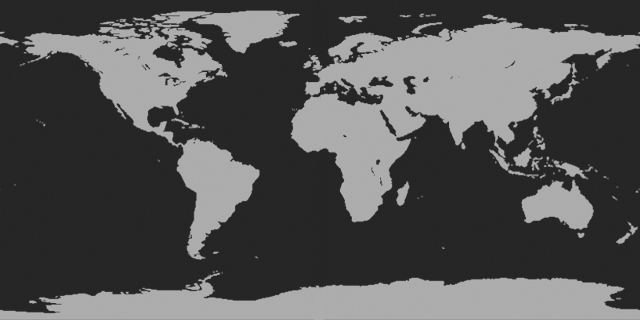
\includegraphics[width=0.8\linewidth]{../starry/maps/earth.jpg}
    \\[1em]
    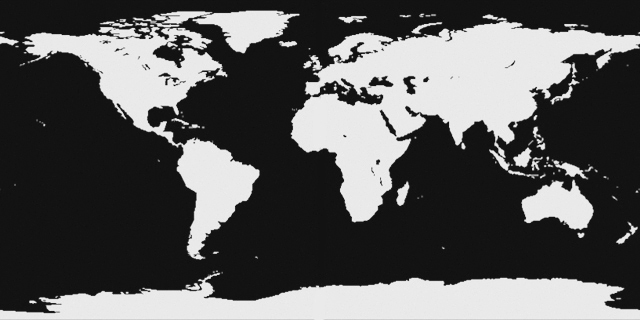
\includegraphics[width=0.85\linewidth]{figures/earth.pdf}
    \caption{\label{fig:earth}
             \python{earth}
             A simple two-color map of the Earth (top) and the
             corresponding tenth-order spherical harmonic expansion,
             rotated about $\xhat$ (bottom).}
    \end{centering}
\end{figure}
%

% ------------------------------------------------------------------------------
\subsection{Computing phase curves}
\label{sec:starryphasecurves}
% ------------------------------------------------------------------------------
%
\begin{figure}[p!]
    \begin{centering}
    \includegraphics[width=\linewidth]{figures/phasecurves.pdf}
    \caption{\label{fig:phasecurves}
             \python{phasecurves}
             Phase curves for the first several spherical harmonics with
             degree $m \ge 0$ rotated about the $x$-axis (blue) and about
             the $y$-axis (orange).
             Odd harmonics with $l > 1$ and harmonics with $m < 0$ are
             in the phase curve null space \citep{CowanFuentesHaggard2013}.}
    \end{centering}
\end{figure}
%
Once a map is instantiated, it is easy to compute its phase curve, \textsf{F}:
%
\begin{lstlisting}[language=Python,firstnumber=last]
F = y.flux(u=u, theta=theta)
\end{lstlisting}
%
where \textsf{u} is the axis of rotation and \textsf{theta} is an array of
angles at which to compute the flux. Note that rotations performed
by \textsf{flux()} are not cumulative; instead, all angles should be specified
relative to the original, unrotated map frame.
%
In Figure~\ref{fig:phasecurves} we plot phasecurves for all spherical harmonics
up to $l_\mathrm{max} = 8$ for rotation about $\xhat$ (blue) and $\yhat$
(orange). As discussed by \citet{CowanFuentesHaggard2013}, harmonics with
odd $l > 1$ and those with $m < 0$ (not plotted) are in the null space and
therefore do not exhibit phase variations.

%

As a second example, we can compute the phase curve of the simplified Earth model
(Figure~\ref{fig:earth}) for rotation about $\yhat$ (its actual spin axis)
by executing
%
\begin{lstlisting}[language=Python,firstnumber=last]
theta = np.linspace(0, 2 * np.pi, 100)
F = y.flux(u=[0, 1, 0], theta=theta)
\end{lstlisting}
%
assuming the \textsf{numpy} package is imported. The variable $\textsf{F}$ is
an array of flux values computed from \eq{phaseint}; we plot this in
Figure~\ref{fig:earthphasecurve}, alongside the phase curves due to each of
the seven individual continents. 
%
\begin{figure}[ht!]
    \begin{centering}
    \includegraphics[width=0.85\linewidth]{figures/earthphasecurve.pdf}
    \caption{\label{fig:earthphasecurve}
             \python{earthphasecurve}
             Phase curve for the Earth rotating about its axis, computed
             from the $l_\mathrm{max} = 10$ expansion from
             Figure~\ref{fig:earth}. The full phase curve is shown in black,
             and the flux due to each of the seven continents is shown as
             the colored curves (see legend).}
    \end{centering}
\end{figure}
%

% ------------------------------------------------------------------------------
\subsection{Computing occultation light curves}
\label{sec:starryoccultation}
% ------------------------------------------------------------------------------

Occultation light curves.\todo{RL}{todo}

% ------------------------------------------------------------------------------
\subsection{Benchmarks}
\label{sec:starrybenchmarks}
% ------------------------------------------------------------------------------

Benchmarks.\todo{RL}{todo}

% ------------------------------------------------------------------------------
\subsection{Speed tests}
\label{sec:starryspeed}
% ------------------------------------------------------------------------------

Speed tests.\todo{RL}{todo}

% ==============================================================================
% ------------------------------------------------------------------------------
% ------------------------------------------------------------------------------
\pagebreak
\section{Conclusions}
\label{sec:conclusions}
% ------------------------------------------------------------------------------
% ------------------------------------------------------------------------------
% ==============================================================================

Write an awesome conclusions section.\todo{RL}{write conclusions}

%


% ==============================================================================
% ------------------------------------------------------------------------------
% ------------------------------------------------------------------------------
\pagebreak
\appendix
\section{Computing the solution vector $\MakeLowercase{s_n}$}
\label{sec:solutionvector}
% ------------------------------------------------------------------------------
% ------------------------------------------------------------------------------
% ==============================================================================

Here we seek a solution to \eq{sn}, which gives the total flux
during an occultation of the $n^\mathrm{th}$ term in the Green's basis
(Equation~\ref{eq:bg}). The primitive integrals $\mathcal{P}$ and
$\mathcal{G}$ in that equation are given by Equations~(\ref{eq:primitiveP})
and (\ref{eq:primitiveQ}), with
$\bvec{G}_n$ defined in \eq{Gn}. Note that all of the terms in \eq{Gn},
with the exception of the $\mu = \nu = 1$ case, are simple polynomials
in $\x$, $\y$, and $\z$, which facilitates their integration.
The $\mu = \nu = 1$ term (corresponding to the $n = 2$ term in the Green's basis)
is more difficult to integrate, but an analytic
solution exists \citep{Pal2012}. It is, however, more convenient
to note that this term corresponds to a surface map given by the polynomial
$I(x, y) = \tilde{g}_2(x, y) = \sqrt{1 - x^2 - y^2}$, which is the same function used
to model linear limb darkening in stars \citep{MandelAgol2002}. We therefore
evaluate this term separately in Appendix~\ref{sec:linearld} below, followed by
the general term in Appendix~\ref{sec:generalterm}.

% ------------------------------------------------------------------------------
\subsection{Linear limb darkening ($n = 2$)}
\label{sec:linearld}
% ------------------------------------------------------------------------------

From \citet{MandelAgol2002}, the total flux visible during the occultation of a
body whose surface map is given by $I(x, y) = \sqrt{1 - \x^2 -\y^2}$ is
%
\begin{align}
    \label{eq:s2}
    s_2 = \frac{2}{3\pi} \left(1 - \frac{3\Lambda}{2} - \Theta(r - b) \right)
\end{align}
%
where $\Theta(\bigdot)$ is the Heaviside step function and
%
\begin{align}
    \label{eq:biglam}
    \Lambda &=
    \begin{dcases}
          -\frac{2}{3}\left(1 - r^2\right)^\frac{3}{2}
          & \qquad b = 0
          %
          \\[1.5em]
          \frac{1}{9 \pi \sqrt{b r}} \Bigg[
                (-3 + 12 r^2 - 10 b^2 r^2 - 6 r^4 + \xi) K(k^2)
                &\\
                \phantom{XXXX}
                - 2 \xi E (k^2)
                + 3 \left(\frac{b + r}{b - r}\right) \Pi\left(1-\frac{1}{(b-r)^2}, k^2\right)
                \Bigg]
          & \qquad k^2 < 1
          %
          \\[1.5em]
          %
          \frac{1}{9 \pi \sqrt{(1{-}b{+}r)(1{+}b{-}r)}} \Bigg[
                2 \left(1 - 5 b^2 + r^2 + (r^2 - b^2)^2\right) K \left(\frac{1}{k^2}\right)
                &\\
                \phantom{XXXXXXXXXXX}
                - 2 \xi k^2 E \left(\frac{1}{k^2}\right)
                &\\
                \phantom{XXXXXXXXXXX}
                + 3 \left(\frac{b + r}{b - r}\right) \Pi\left(\frac{1}{k^2 - \frac{1}{4 b r}}, \frac{1}{k^2}\right)
                \Bigg]
          & \qquad k^2 \ge 1
    \end{dcases}
\end{align}
%
with
%
\begin{align}
    \label{eq:k2}
    \xi &= 2 b r (4 - 7 r^2 - b^2) \nonumber \\
    k^2 &= \frac{1 - r^2 - b^2}{4 b r}
    \quad.
\end{align}
%
In the expressions above, $K(\bigdot)$, $E(\bigdot)$, and $\Pi(\bigdot)$
are the complete elliptic integrals of the first, second kind, and third kind,
respectively, defined as
%
\begin{align}
    \label{eq:elliptic}
    K(k^2) &\equiv \int_0^{\frac{\pi}{2}} \frac{\dd \varphi}{\sqrt{1 - k^2 \sin^2 \varphi}}
    \nonumber \\[0.5em]
    E(k^2) &\equiv \int_0^{\frac{\pi}{2}} \sqrt{1 - k^2 \sin^2 \varphi} \, \dd \varphi
    \nonumber \\[0.5em]
    \Pi(n^2, k^2) &\equiv \int_0^{\frac{\pi}{2}} \frac{\dd \varphi}{(1 - n^2 \sin^2 \varphi)\sqrt{1 - k^2 \sin^2 \varphi}}
    \quad.
\end{align}

% ------------------------------------------------------------------------------
\subsection{All other terms}
\label{sec:generalterm}
% ------------------------------------------------------------------------------

We evaluate all other terms in $s_n$ by integrating the primitive integrals of
$\bvec{G}_n$. These are given by
%
\begin{align}
    \label{eq:PGn}
    \mathcal{P}(\bvec{G}_n) &=
    \begin{dcases}
        %
        +\int\displaylimits_{\pi - \phi}^{2\pi + \phi}
            (r c_\varphi)^{\frac{\mu+2}{2}}
            (b + r s_\varphi)^{\frac{\nu}{2}}
            r c_\varphi
            \, \dd\varphi
            %
            & \qquad \nu \, \mathrm{even}
        \\[1em]
        %
        -\int\displaylimits_{\pi - \phi}^{2\pi + \phi}
            (r c_\varphi)^{l-2}
            (1 {-} r^2 {-} b^2 {-} 2 b r s_\varphi)^{\frac{3}{2}}
            r s_\varphi
            \, \dd\varphi
            %
            & \qquad \nu \, \mathrm{odd}, \,
                     \mu = 1, \,
                     l \, \mathrm{even}
        \\[1em]
        %
        -\int\displaylimits_{\pi - \phi}^{2\pi + \phi}
            (r c_\varphi)^{l-3}
            (b + r s_\varphi)
            (1 {-} r^2 {-} b^2 {-} 2 b r s_\varphi)^{\frac{3}{2}}
            r s_\varphi
            \, \dd\varphi
            %
            & \qquad \nu \, \mathrm{odd}, \,
                     \mu = 1, \,
                     l \, \mathrm{odd}
        \\[1em]
        %
        +\int\displaylimits_{\pi - \phi}^{2\pi + \phi}
            (r c_\varphi)^{\frac{\mu-3}{2}}
            (b + r s_\varphi)^{\frac{\nu-1}{2}}
            (1 {-} r^2 {-} b^2 {-} 2 b r s_\varphi)^{\frac{3}{2}}
            r c_\varphi
            \, \dd\varphi
            & \qquad \mathrm{otherwise}
    \end{dcases}
%
\intertext{and}
%
    \nonumber \\
    \label{eq:QGn}
    \mathcal{Q}(\bvec{G}_n) &=
    \begin{dcases}
        %
        +\int\displaylimits_{\pi - \lambda}^{2\pi + \lambda}
            c_\varphi^{\frac{\mu+2}{2}}
            s_\varphi^{\frac{\nu}{2}}
            c_\varphi
            \, \dd\varphi
            %
            & \qquad\qquad \nu \, \mathrm{even}
        \\[1em]
        %
        \phantom{XXXXX}0
            & \qquad\qquad \mathrm{otherwise,}
    \end{dcases}
\end{align}
%
%
where we have used the fact that the line integral of any function
proportional to $\z$ taken along the limb of the occulted planet
(where $\z = \sqrt{1-\x^2-\y^2} = 0$) is zero.
%
For convenience, let us introduce the expressions
%
\begin{align}
    \label{eq:Hun}
    \mathcal{H}_{u,n}^\nu(\xi, \beta, \rho) &=
    \begin{dcases}
        \int\displaylimits_{\pi - \xi}^{2\pi + \xi}
            c_\varphi^u
            s_\varphi^n
            \, \dd\varphi
            & \qquad \nu \, \mathrm{even}
        \\[1em]
        \int\displaylimits_{\pi - \xi}^{2\pi + \xi}
            c_\varphi^u
            s_\varphi^n
            (1 - \rho^2 - \beta^2 - 2 \beta \rho s_\varphi)^{\frac{3}{2}}
            \, \dd\varphi
            & \qquad \nu \, \mathrm{odd}
    \end{dcases}
\end{align}
%
and
%
\begin{align}
    \label{eq:Iuv}
    \mathcal{I}_{u,v}^\nu(\xi, \beta, \rho) &=
        \sum\displaylimits_{n=0}^{v}
        {v \choose n}
        \left(\frac{\beta}{\rho}\right)^{v-n}
        \mathcal{H}_{u, n}^\nu (\xi, \beta, \rho)
        \quad.
\end{align}
%
With some algebra, we may therefore write
%
\begin{align}
    \label{eq:PGnI}
    \mathcal{P}(\bvec{G}_n) &=
    \begin{dcases}
        %
        r^{l+2} \mathcal{I}_{\frac{\mu+4}{2}, \frac{\nu}{2}}^\nu (\phi, b, r)
            %
            & \qquad \nu \, \mathrm{even}
        \\[1em]
        %
        b r^{l-2} \mathcal{I}_{l-2, 0}^\nu (\phi, b, r)
        - r^{l-1} \mathcal{I}_{l-2,1}^\nu (\phi, b, r)
            %
            & \qquad \nu \, \mathrm{odd}, \,
                     \mu = 1, \,
                     l \, \mathrm{even}
        \\[1em]
        %
        b r^{l-2} \mathcal{I}_{l-3, 1}^\nu (\phi, b, r)
        - r^{l-1} \mathcal{I}_{l-3,2}^\nu (\phi, b, r)
            %
            & \qquad \nu \, \mathrm{odd}, \,
                     \mu = 1, \,
                     l \, \mathrm{odd}
        \\[1em]
        %
        r^{l-1} \mathcal{I}_{\frac{\mu-1}{2}, \frac{\nu-1}{2}}^\nu (\phi, b, r)
            & \qquad \mathrm{otherwise}
    \end{dcases}
%
\intertext{and}
%
    \nonumber \\
    \label{eq:QGnI}
    \mathcal{Q}(\bvec{G}_n) &=
    \begin{dcases}
        %
        \mathcal{I}_{\frac{\mu+4}{2}, \frac{\nu}{2}}^\nu (\lambda, 0, 1)
            %
            & \qquad\qquad \nu \, \mathrm{even}
        \\[1em]
        %
        \phantom{XXX}0
            & \qquad\qquad \mathrm{otherwise.}
    \end{dcases}
\end{align}
%
The solution to the occultation problem is therefore a matter of finding
expressions for $\mathcal{H}_{u, n}^{\nu}$ (Equation~\ref{eq:Hun}):
\\

\noindent \textbf{\underline{Case 1: $\nu$ even}}\\

\noindent For even $\nu$, $\mathcal{H}_{u, n}^{\nu}$ evaluates to terms containing
only sines and cosines of $\xi$. \citet{Pal2012} derived simple recurrence relations
for these terms:
%
\begin{align}\
    \label{eq:Huneven}
    \mathcal{H}_{u,n}^{\nu}(\xi, \beta, \rho) &=
    \begin{dcases}
        0
        & \qquad u \ \mathrm{odd}
        %
        \\[0.5em]
        %
        2\xi + \pi
        & \qquad u = n = 0
        %
        \\[0.5em]
        %
        -2\cos\xi
        & \qquad u = 0, n = 1
        %
        \\[0.5em]
        %
        \frac{2}{u + n}
        (\cos\xi)^{u-1} (\sin\xi)^{n+1} +
        \frac{u-1}{u+n} \mathcal{H}_{u-2,n}^{\nu}(\xi, \beta, \rho)
        & \qquad u \ge 2
        %
        \\[0.5em]
        %
        -\frac{2}{u + n}
        (\cos\xi)^{u+1} (\sin\xi)^{n-1} +
        \frac{n-1}{u+n} \mathcal{H}_{u,n-2}^{\nu}(\xi, \beta, \rho)
        & \qquad n \ge 2
        \quad.
        %
    \end{dcases}
\end{align}
\\

\noindent \textbf{\underline{Case 2: $\nu$ odd}}\\

\noindent When $\nu$ is odd, $\mathcal{Q}(\bvec{G}_n) = 0$ and
we need only compute $\mathcal{P}(\bvec{G}_n)$, for which
$\xi = \phi$, $\beta = b$, and $\rho = r$. However,
because of the term raised to the $\nicefrac{3}{2}$ power in
\eq{Hun} for odd $\nu$, the integral becomes significantly more
difficult to compute. With some algebraic manipulation, and using
recurrence relations for expressions with integrands
of the form $\cos^p\varphi\sin^q\varphi (1 - \kappa^2 \sin^2 \varphi)^\frac{3}{2}$
\citep{Gradshteyn1994}, we may write
%
\begin{align}
    \label{eq:Hunodd}
    \mathcal{H}_{u,n}^{\nu}(\phi, b, r) &=
        2^{u+3} (b r)^\frac{3}{2}
        \sum\displaylimits_{m=0}^n
            {n \choose m}\left(-1\right)^{m-n-u}\mathcal{J}_{u + 2m, u + 2n - 2m}(k^2)
\end{align}
%
where
%
\begin{align}
    \label{eq:Jpq}
    \mathcal{J}_{p, q} (k^2) &=
    \begin{dcases}
        %
        0 & \qquad p\ \mathrm{odd} \ \mathrm{or} \ q\ \mathrm{odd}\\[0.5em]
        %
        \frac{d_1 \mathcal{J}_{p,q-2}(k^2) + d_2 \mathcal{J}_{p,q-4}(k^2)}
             {p + q + 3}
        & \qquad q \ge 4 \\[0.5em]
        %
        \frac{d_3 \mathcal{J}_{p-2,q}(k^2) + d_4 \mathcal{J}_{p-4,q}(k^2)}
             {p + q + 3}
         & \qquad p \ge 4
    \end{dcases}
\end{align}
%
with
%
\begin{align}
    d_1 &= q + 2 + (p + q - 2)(1 - k^2) \nonumber \\
    d_2 &= (3 - q)(1 - k^2) \nonumber \\
    d_3 &= 2 p + q - (p + q - 2)(1 - k^2) \nonumber \\
    d_4 &= (3 - p) + (p - 3)(1 - k^2)
\end{align}
%
and $k^2$ defined as in \eq{k2}.
%
These recurrence relations require four initial conditions:
%
\begin{align}
    \mathcal{J}_{0,0}(k^2) &= \frac{8-12k^2}{3}\mathcal{E}_1(k^2) + \frac{-8 + 16k^2}{3}\mathcal{E}_2(k^2) \nonumber \\[1em]
    \mathcal{J}_{0,2}(k^2) &= \frac{8-24k^2}{15}\mathcal{E}_1(k^2) + \frac{-8 + 28k^2 + 12k^4}{15}\mathcal{E}_2(k^2) \nonumber \\[1em]
    \mathcal{J}_{2,0}(k^2) &= \frac{32 - 36k^2}{15}\mathcal{E}_1(k^2) + \frac{-32 + 52k^2 - 12k^4}{15}\mathcal{E}_2(k^2) \nonumber \\[1em]
    \mathcal{J}_{2,2}(k^2) &= \frac{32-60k^2+12k^4}{105}\mathcal{E}_1(k^2) + \frac{-32 + 76 k^2 - 36 k^4 + 24 k^6}{105}\mathcal{E}_2(k^2)
    \quad,
\end{align}
%
where
%
\begin{align}
    \label{eq:E1}
    \mathcal{E}_1(k^2) &=
    \begin{dcases}
        (1-k^2) K \left(k^2\right) & \qquad k^2 < 1 \\[0.5em]
        \frac{1-k^2}{\sqrt{k^2}} K \left(\frac{1}{k^2}\right) & \qquad k^2 \ge 1
    \end{dcases}
    \\[0.5em]
\intertext{and}
    \label{eq:E2}
    \mathcal{E}_2(k^2) &=
    \begin{dcases}
        E \left(k^2\right) & \qquad k^2 < 1 \\[0.5em]
        k E \left(\frac{1}{k^2}\right)
            + \frac{1-k^2}{\sqrt{k^2}} K \left(\frac{1}{k^2}\right)
          & \qquad k^2 \ge 1
          \quad.
    \end{dcases}
\end{align}
%
Interestingly, the elliptic integrals in the expressions above are exactly
the same as the ones used to evaluate the $s_2$ term (Equation~\ref{eq:biglam}),
so these need only be evaluated \emph{once} when computing the occultation flux of
a map of arbitrary order. Thanks to the recurrence relations, all other operations
required to evaluate the integrals for odd $\mu$ are elementary, making the
computation of $s_n$ fast.

Note, finally, that the expressions above diverge when $b = 0$,
since $k^2 \rightarrow \infty$.
In this case, the integral in \eq{Hun} simplifies:
%
\begin{align}
    \mathcal{H}_{u,n}^{\nu}(\phi, 0, r) = (1 - r^2)^\frac{3}{2} \mathcal{H}_{u,n}^{\nu + 1}(\phi, 0, r)
\end{align}
%
with $\mathcal{H}_{u,n}^{\nu + 1}$ given by \eq{Huneven}.

%

\begin{center}
\begin{longtable}{cll}
\caption{Symbols used in this paper} \label{tab:symbols} \\
%
\toprule
\multicolumn{1}{c}{\textbf{Symbol}} &
\multicolumn{1}{c}{\textbf{Definition}} &
\multicolumn{1}{c}{\textbf{Reference}} \\
\midrule
\endfirsthead
%
\multicolumn{3}{c}%
{{\bfseries \tablename\ \thetable{} --} continued from previous page} \\
\toprule
\multicolumn{1}{c}{\textbf{Symbol}} &
\multicolumn{1}{c}{\textbf{Definition}} &
\multicolumn{1}{c}{\textbf{Reference}} \\
\midrule
\endhead
\bottomrule
%
\endfoot
%
\bottomrule
\endlastfoot
%
$A_{lm}$        & Legendre function normalization       & \eq{alm} \\
$\bvec{A}$      & Change of basis matrix:
                  spherical harmonics to Greens
                  polynomials                           & \eq{A} \\
$\AOne$         & Change of basis matrix:
                  spherical harmonics to polynomials    & \S\ref{sec:polybasis} \\
$\ATwo$         & Change of basis matrix:
                  polynomials to Greens polynomials     & \S\ref{sec:greensbasis} \\
$b$             & Impact parameter in units of occulted
                  body's radius                         & \S\ref{sec:occultations} \\
$B_{lm}^{jk}$   & Spherical harmonic normalization      & \eq{blmjk} \\

$c_{\bigdot}$   & $\cos(\bigdot)$                       & \\
$C_{pq}^k$      & Expansion coefficient for
                  $\z(\x, \y)$                          & \eq{ckpq} \\
$\bvec{D}^l$    & Rotation matrix for the
                  complex spherical harmonics
                  of order $l$                          & \eq{dl} \\
$\bvec{D}\,\wedge$
                & Exterior derivative                   & \eq{extderiv} \\
$E(\bigdot)$    & Complete elliptic integral of the
                  second kind                           & \eq{elliptic} \\
$\mathcal{E}_1$ & First elliptic function               & \eq{E1} \\
$\mathcal{E}_2$ & Second elliptic function              & \eq{E2} \\
$F$             & Total flux seen by observer           & \eq{starry} \\
$\gbasis$       & Green's basis                         & \eq{bg} \\
$\bvec{g}$      & Vector in the basis $\gbasis$         & \\
$\bvec{G}_n$    & Anti-exterior derivative of the
                  $n^\mathrm{th}$
                  term in the Green's basis             & \eq{Gn} \\
$\mathcal{H}_{u,n}^{\nu}$
                & Occultation integral                  & \eq{Hun} \\
$I$             & Specific intensity, $I(\x, \y)$       & \eq{I} \\
$\mathcal{I}_{u,v}^{\nu}$
                & Occultation integral                  & \eq{Iuv} \\
$j$             & Dummy index                           & \\
$\mathcal{J}_{p,q}$
                & Occultation integral                  & \eq{Jpq} \\
$k$             & Dummy index                           & \\
$k^2$           & Elliptic parameter                    & \eq{k2} \\
$K(\bigdot)$    & Complete Elliptic integral of the
                  first kind                            & \eq{elliptic} \\
$l$             & Spherical harmonic order              & \eq{lm} \\
$m$             & Spherical harmonic degree             & \eq{lm} \\
$n$             & Surface map vector index,
                  $n = l^2 + l + m$                     & \eq{n} \\
$p$             & Dummy index                           & \\
$\bar{P}$       & Normalized associated Legendre
                  function                              & \eq{plm} \\
$\pbasis$       & Polynomial basis                      & \eq{bp} \\
$\bvec{p}$      & Vector in the basis $\pbasis$         & \\
$\bvec{P}$      & Cartesian axis-angle rotation matrix  & \eq{rotP} \\
$\mathcal{P}$   & Primitive integral along perimiter
                  of occultor                           & \eq{primitiveP} \\
$q$             & Dummy index                           & \\
$\bvec{Q}$      & Cartesian Euler angle rotation matrix & \eq{rotQ} \\
$\mathcal{Q}$   & Primitive integral along perimiter
                  of occulted body                      & \eq{primitiveQ} \\
$r$             & Occultor radius in units of occulted
                  body's radius                         & \S\ref{sec:occultations} \\
$\bvec{r}$      & Phase curve solution vector           & \eq{rn} \\
$\bvec{R}$      & Rotation matrix for the real
                  spherical harmonics                   & \eq{rblockdiag} \\
$\bvec{R}^l$    & Rotation matrix for the real
                  spherical harmonics of order $l$      & \eq{rl} \\
$s_{\bigdot}$   & $\sin(\bigdot)$                       & \\
$\bvec{s}$      & Occultation light curve solution
                  vector                                & \eq{rn} \\
$\bvec{u}$      & Unit vector corresponding to the
                  axis of rotation                      & \S\ref{sec:axisangle} \\
$\bvec{U}$      & Complex to real spherical harmonics
                  transform matrix                      & \eq{U} \\
$\x$            & Cartesian coordinate                  & \eq{xyz} \\
$\y$            & Cartesian coordinate                  & \eq{xyz} \\
$Y_{l,m}$       & Spherical harmonic of order $l$
                  and degree $m$                        & \eq{ylm0} \\
$\ybasis$       & Spherical harmonic basis              & \eq{by} \\
$\bvec{y}$      & Vector in the basis $\ybasis$         & \\
$\z$            & Cartesian coordinate,
                  $z = \sqrt{1 - \x^2 - \y^2}$          & \eq{xyz} \\
%
$\alpha$        & Euler angle ($\zhat$ rotation)        & \S\ref{sec:euler} \\
$\beta$         & Euler angle ($\yhat$ rotation)        & \S\ref{sec:euler} \\
$\gamma$        & Euler angle ($\zhat$ rotation)        & \S\ref{sec:euler} \\
$\theta$        & Polar angle                           & \eq{ylmtp} \\
                & Spherical harmonic rotation angle     & \S\ref{sec:axisangle} \\
$\Theta$        & Heaviside step function               & \eq{biglam} \\
$\lambda$       & Angular position of intersection point
                  between occulted and occultor         & \eq{lambda} \\
$\Lambda$       & \citet{MandelAgol2002} function       & \eq{biglam} \\
$\mu$           & $l - m$                               & \eq{munu} \\
$\nu$           & $l + m$                               & \eq{munu} \\
$\xi$           & Function of $b$ and $r$               & \ref{eq:k2} \\
$\Pi(\bigdot,\bigdot)$
                & Complete elliptic integral of the
                  third kind                            & \eq{elliptic} \\
$\phi$          & Spherical harmonic azimuthal angle    & \eq{ylmtp} \\
                & Angular position of intersection point
                  between occulted and occultor         & \eq{phi} \\
$\varphi$       & Dummy integration variable            & \\
$\omega$        & Angular position of occultor          & \eq{zrot}
%
\end{longtable}
\end{center}


\bibliography{starry}

\end{document}
